\documentclass{article}
\usepackage{amsmath, amssymb, amsthm, graphicx}
\usepackage[export]{adjustbox}

\title{Chapter 2 Section 3}
\author{Andrew Taylor}
\date{April 11 2022}
\newtheorem{theorem}{Theorem}
\newtheorem{problem}{Problem}
\newtheorem*{solution}{Solution}

\begin{document}
\maketitle

\begin{problem}
Calculate the matrix product

\begin{align*}
\begin{bmatrix}
6 & 7 \\
8 & 9
\end{bmatrix}
\begin{bmatrix}
1 & 2 \\
3 & 5
\end{bmatrix}
\end{align*}
\end{problem}

\begin{solution}
\begin{align*}
\begin{bmatrix}
6 & 7 \\
8 & 9
\end{bmatrix}
\begin{bmatrix}
1 & 2 \\
3 & 5
\end{bmatrix}
&= 
\begin{bmatrix}
6*1 + 7*3 & 6*2 + 7*5 \\
8*1 + 9*3 & 8*2 + 9*5
\end{bmatrix} \\
&= 
\begin{bmatrix}
27 & 47 \\
35 & 61
\end{bmatrix}
\end{align*}
\end{solution}

\begin{problem}
Compute the products BA and AB for 

\begin{align*}
A = \begin{bmatrix}0 & 1 \\ 1 & 0 \end{bmatrix}
\end{align*}

\begin{align*}
B = \begin{bmatrix}-1 & 0 \\ 0 & 1 \end{bmatrix} 
\end{align*}

Interpret your answers geometrically, as composites of linear transformation.
\end{problem}

\begin{solution}
Let $T_{A}(\vec{x}) = A\vec{x}$ and $T_{B}(\vec{y}) = B\vec{y}$. We can write 

\begin{align*}
A &= \begin{bmatrix}0 & 1 \\ 1 & 0 \end{bmatrix} = \begin{bmatrix} T_{A} (e_{1}) & T_{A} (e_{2}) \end{bmatrix} \\
B &= \begin{bmatrix}-1 & 0 \\ 0 & 1 \end{bmatrix} = \begin{bmatrix} T_{B} (e_{1}) & T_{B} (e_{2}) \end{bmatrix}
\end{align*}

Thus 

\begin{align*}
T_{A}(\vec{e_{1}}) &= \begin{bmatrix} 0 \\ 1 \end{bmatrix}, \,T_{A}(\vec{e_{2}}) = \begin{bmatrix} 1 \\ 0 \end{bmatrix} \\
T_{B}(\vec{e_{1}}) &= \begin{bmatrix} -1 \\ 0 \end{bmatrix}, \, T_{B}(\vec{e_{2}}) = \begin{bmatrix} 0 \\ 1 \end{bmatrix}
\end{align*}

We see that $T_{A}$ is a reflection about the line $y = x$. In other words, $T_{A}$ is a reflection about the line spanned by the vector $\vec{w} = \begin{bmatrix} 1 \\ 1 \end{bmatrix}$. \\

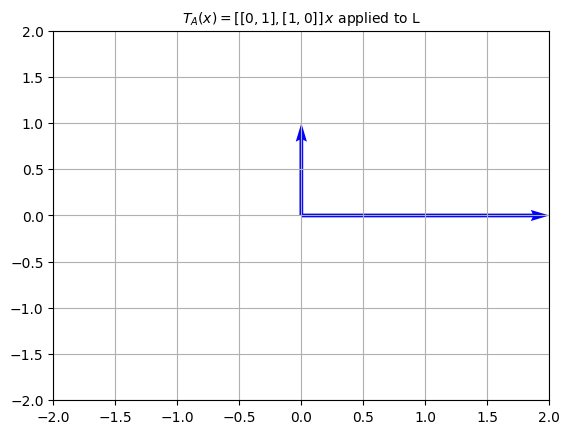
\includegraphics[scale=0.5, center]{Lreflectyeqx} 

We see that $T_{B}$ is a reflection about the line $x = 0$. In other words, $T_{B}$ is a reflection about the line spanned by the vector $\vec{w} = \begin{bmatrix} 0 \\ 1 \end{bmatrix}$. \\

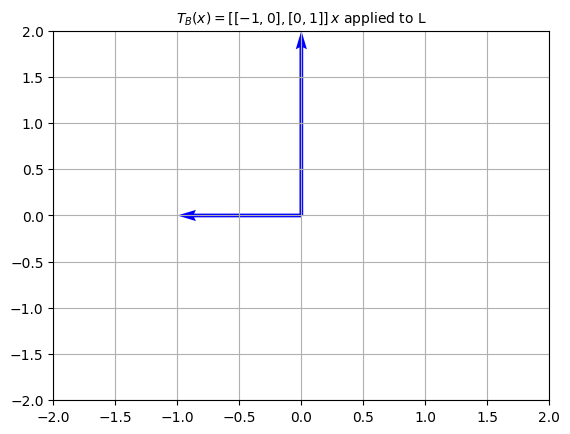
\includegraphics[scale=0.5, center]{Lreflectxeq0} 

Now let's compute the products BA and AB.

\begin{align*}
BA &= \begin{bmatrix}-1 & 0 \\ 0 & 1 \end{bmatrix} 
\begin{bmatrix}0 & 1 \\ 1 & 0 \end{bmatrix} \\
&= \begin{bmatrix}0 & -1 \\ 1 & 0 \end{bmatrix} 
\end{align*}

The product BA is a rotation matrix that rotates a vector ninety degrees counterclockwise. \\

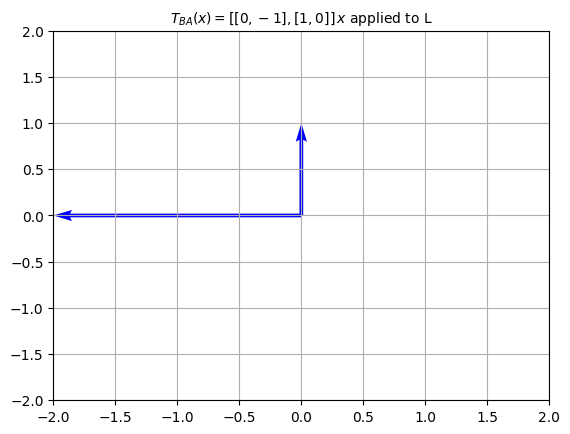
\includegraphics[scale=0.5, center]{Lrot90ccw} 

\begin{align*}
AB &= \begin{bmatrix}0 & 1 \\ 1 & 0 \end{bmatrix} 
\begin{bmatrix}-1 & 0 \\ 0 & 1 \end{bmatrix} \\
&= \begin{bmatrix}0 & 1 \\ -1 & 0 \end{bmatrix} 
\end{align*}

The product AB is a rotation matrix that rotates a vector ninety degrees clockwise. \\
\end{solution}

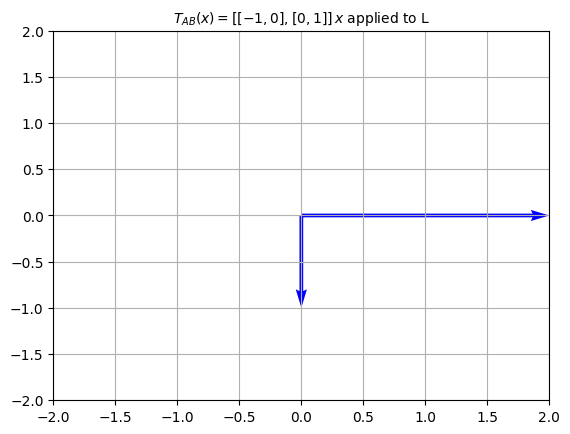
\includegraphics[scale=0.5, center]{Lrot90cw} 

\begin{problem}
Multiply the block matrices

\begin{align*}
& \left(
\begin{array}{@{}cc|c@{}}
0 & 1 & -1 \\ 1 & 0 & 1
\end{array}
\right)
\left(
\begin{array}{@{}cc|c@{}}
1 & 2 & 3 \\ 4 & 5 & 6 \\ \hline 7 & 8 & 9
\end{array}
\right) 
\end{align*}

Afterwards, compute the product without a partition and see if you get the same result.
\end{problem}

\begin{solution}
\begin{align*}
& \left(
\begin{array}{@{}cc|c@{}}
0 & 1 & -1 \\ 1 & 0 & 1
\end{array}
\right)
\left(
\begin{array}{@{}cc|c@{}}
1 & 2 & 3 \\ 4 & 5 & 6 \\ \hline 7 & 8 & 9
\end{array}
\right) \\
&= \left(
\begin{array}{@{}c|c@{}}
\begin{bmatrix}0 & 1 \\ 1 & 0 \end{bmatrix} \begin{bmatrix}1 & 2 \\ 4 & 5 \end{bmatrix} + \begin{bmatrix} -1 \\ 1 \end{bmatrix} \begin{bmatrix} 7 & 8 \end{bmatrix} &
\begin{bmatrix}0 & 1 \\ 1 & 0 \end{bmatrix} \begin{bmatrix} 3 \\ 6 \end{bmatrix} + \begin{bmatrix} -1 \\ 1 \end{bmatrix} \begin{bmatrix} 9 \end{bmatrix} \\
\end{array} 
\right) \\
&=
\left(
\begin{array}{@{}c|c@{}} 
\begin{bmatrix}4 & 5 \\ 1 & 2 \end{bmatrix} + \begin{bmatrix}-7 & -8 \\ 7 & 8 \end{bmatrix} & \begin{bmatrix} 6 \\ 3 \end{bmatrix} + \begin{bmatrix} -9 \\ 9 \end{bmatrix}
\end{array}
\right) \\
&=
\left(
\begin{array}{@{}c|c@{}} 
\begin{bmatrix}-3 & -3 \\ 8 & 10 \end{bmatrix} & \begin{bmatrix} -3 \\ 12 \end{bmatrix}
\end{array}
\right) \\
&=
\left(
\begin{array}{@{}cc|c@{}} 
-3 & -3 & -3 \\ 8 & 10 & 12
\end{array}
\right)
\end{align*}

Now let's compute the product without a partition.

\begin{align*}
& \begin{bmatrix}0 & 1 & -1 \\ 1 & 0 & 1 \end{bmatrix}
\begin{bmatrix}1 & 2 & 3 \\ 4 & 5 & 6 \\ 7 & 8 & 9 \end{bmatrix} \\
&= \begin{bmatrix}4 - 7 & 5 - 8 & 6 - 9 \\ 1 + 7 & 2 + 8 & 3 + 9 \end{bmatrix} \\
&= \begin{bmatrix}-3 & -3 & -3 \\ 8 & 10 & 12 \end{bmatrix}
\end{align*}

We get the same result.

\end{solution}

In the following problems, multiply the matrices and describe the linear transformations geometrically.

\begin{problem}
\begin{align*}
\begin{bmatrix}
1 & 1 \\ 0 & 1
\end{bmatrix}
\begin{bmatrix}
1 & 2 \\ 3 & 4
\end{bmatrix}
\end{align*}
\end{problem}

\begin{solution}
The first matrix is a horizontal shear with k = 1.

\begin{align*}
& \begin{bmatrix}
1 & 1 \\ 0 & 1
\end{bmatrix}
\begin{bmatrix}
1 & 2 \\ 3 & 4
\end{bmatrix} \\
&= 
\begin{bmatrix}
4 & 6 \\ 3 & 4
\end{bmatrix} 
\end{align*}
\end{solution}

\begin{problem}
\begin{align*}
\begin{bmatrix}
1 & -1 \\ 0 & 2 \\ 2 & 1
\end{bmatrix}
\begin{bmatrix}
3 & 2 \\ 1 & 0
\end{bmatrix}
\end{align*}
\end{problem}

\begin{solution}
Let A be a n by p matrix and let B be a q by m matrix. The product of a matrix AB is defined if and only if p = q. \\

In the matrices below, p = q, so the product of the matrices is defined.

\begin{align*}
& \begin{bmatrix}
1 & -1 \\ 0 & 2 \\ 2 & 1
\end{bmatrix}
\begin{bmatrix}
3 & 2 \\ 1 & 0
\end{bmatrix} \\
&= \begin{bmatrix}
3 - 1 & 2 - 0 \\ 2 & 0 \\ 6 + 1 & 4
\end{bmatrix} \\
&= \begin{bmatrix}
2 & 2 \\ 2 & 0 \\ 7 & 4
\end{bmatrix} 
\end{align*}
\end{solution}

\begin{problem}
\begin{align*}
\begin{bmatrix}
1 & 2 & 3 \\ 4 & 5 & 6
\end{bmatrix}
\begin{bmatrix}
1 & 2 \\ 3 & 4
\end{bmatrix}
\end{align*}
\end{problem}

\begin{solution}
The matrix product is not defined, since the number of columns in the first matrix (3) does not equal the number of rows in the second matrix (2)
\end{solution}

\begin{problem}
\begin{align*}
\begin{bmatrix}
1 & -1 \\ -2 & 2
\end{bmatrix}
\begin{bmatrix}
7 & 5 \\ 3 & 1
\end{bmatrix}
\end{align*}
\end{problem}

\begin{solution}
\begin{align*}
& \begin{bmatrix}
1 & -1 \\ -2 & 2
\end{bmatrix}
\begin{bmatrix}
7 & 5 \\ 3 & 1
\end{bmatrix} \\
&= \begin{bmatrix}
7-3 & 5-1 \\ -14+6 & -10 + 2
\end{bmatrix} \\
&= \begin{bmatrix}
4 & 4 \\ -8 & -8
\end{bmatrix} 
\end{align*}
\end{solution}

\end{document}